% !TEX root = MAIN.tex


\section{GSL - libgcsp}
\label{sec:caseStudies:GSL:libgcsp}

\subsection{Overview of the case study}

The GomSpace CSP library (libgscsp) is a GomSpace extension to the open source CubeSat Space Protocol library.
The GomSpace CSP library provides:
\begin{itemize}
\item convenience wrapping of CSP functionality, primarily initialization.
\item definition of standard CSP ports (used by other GomSpace products).
\item connecting low-level drivers (e.g. CAN, I2C from Embed library) with CSP interfaces 
\item generic CSP service dispatcher, forwards incoming connections to service handlers.
\end{itemize}

The libgscsp contains a GomSpace branch (https://github.com/GomSpace/libcsp) of the open source libcsp (https://github.com/libcsp/libcsp), located in the subfolder lib/libcsp. The two libcsp branches are kept as identical as possible, as features specific to GomSpace are placed in libgscsp.

Details about libgscsp are provided in the document \emph{gs-man-nanosoft-ms100-command-and-management-sdk-3.6.2-1-g67fe6e1.pdf} uploaded on Alfresco.

\DONE{Add details about size}

The size of libgscsp is 1\,497 LOC, %include 306, src 1776+15 = total = 1497
while libcsp is 8\,339 LOC. % 6789 + 1550


\subsection{Code Coverage}
\label{subsec:csp_coverage}

\DONE{Can we provide separate information about the code coverage for libgscsp (no libcsp branch) and for libcsp branch?}

% !TEX root = ../MAIN.tex

\begin{table}[h]

\footnotesize
\parbox{.45\linewidth}{
\centering
\begin{tabular}{|l|l|}
\hline
\textbf{Coverage Type} & \textbf{Coverage Rate} \\
\hline
Statement     & 58.4\% (390 of 668 statements)\\
Functions     & 71.4\% (50 of 70 functions)\\
Branches      & 41.2\% (165 of 400 branches)\\
\hline
\end{tabular}
\caption{libgscsp code coverage.}
\label{table:libgscsp_coverage}
}
\hfill
\parbox{.45\linewidth}{
\centering
\begin{tabular}{|l|l|}
\hline
\textbf{Coverage Type} & \textbf{Coverage Rate} \\
\hline
Statement     & 64.1\% (2112 of 3297 statements)\\
Functions     & 72.5\% (248 of 342 functions)\\
Branches      & 44.9\% (989 of 2201 branches)\\
\hline
\end{tabular}
\caption{libcsp code coverage.}
\label{table:libcsp_coverage}
}
\end{table}	

\begin{enumerate}
	\item \textbf{libgscsp}

	Table~\ref{table:libgscsp_coverage} provides the code coverage information of the libgscsp unit test suite for the GSL extension to the CSP library. Given the code coverage, we focus our analysis to the following subset of components:

	\begin{itemize}
	 	\item src/clock.c
	 	\item src/commands.c
	 	\item src/conn.c
	 	\item src/csp.c
	 	\item src/error.c
	 	\item src/log.c
	 	\item src/router.c
	 	\item src/service\_dispatcher.c
	 	\item src/service\_handler.c
	 	\item src/linux/command\_line.c

	 \end{itemize} 

	\item \textbf{libcsp (GSL branch)}

	Table~\ref{table:libcsp_coverage} presents the code coverage of the libgscsp unit test suite for the GSL branch of the CSP library.  Given the code coverage, we focus our mutation analysis on the following subset of components:

	\begin{itemize}
		\item src/arch/csp\_time.c
		\item src/arch/csp\_system.c
		\item src/arch/posix/csp\_thread.c
		\item src/arch/posix/csp\_semaphore.c
		\item src/arch/posix/csp\_malloc.c
		\item src/arch/posix/csp\_queue.c
		\item src/arch/posix/csp\_time.c
		\item src/arch/posix/pthread\_queue.c
		\item src/arch/posix/csp\_system.c
		\item src/crypto/csp\_sha1.c
		\item src/crypto/csp\_hmac.c
		\item src/crypto/csp\_xtea.c
		\item src/interfaces/csp\_if\_lo.c
		\item src/rtable/csp\_rtable.c
		\item src/rtable/csp\_rtable\_cidr.c
		\item src/rtable/csp\_rtable\_static.c
		\item src/transport/csp\_rdp.c
		\item src/transport/csp\_udp.c
		\item src/csp\_sfp.c
		\item src/csp\_debug.c
		\item src/csp\_service\_handler.c
		\item src/csp\_crc32.c
		\item src/csp\_io.c
		\item src/csp\_qfifo.c
		\item src/csp\_iflist.c
		\item src/csp\_endian.c
		\item src/csp\_route.c
		\item src/csp\_buffer.c
		\item src/csp\_port.c
		\item src/csp\_conn.c
		\item src/csp\_init.c
		\item src/csp\_services.c
	\end{itemize}


\end{enumerate}



\subsection{Code-driven mutation testing}

\DONE{Clarify which components we mutate}

We have seen that a mutant can be killed only if it is covered by at least one test case. For this reason, the code-driven mutation testing process in libgscsp will target all the components covered by the libgscsp unit test suite. Thus, we include all the components described in the previous Section~\ref{subsec:csp_coverage} for both the libgscsp and the libcsp.

\subsection{Data-driven mutation testing}

\DONE{We should indicate the functions we mutate.}

The data-driven mutation testing process in libgscsp will target the data packet transferred between the server and the client using the CSP protocol. Specifically, the mutations will affect the header of the packet, in general the routing information (see Figure~\ref{fig:csp_packet}), and the payload of the packet.

\begin{figure}[h]
  \centering
    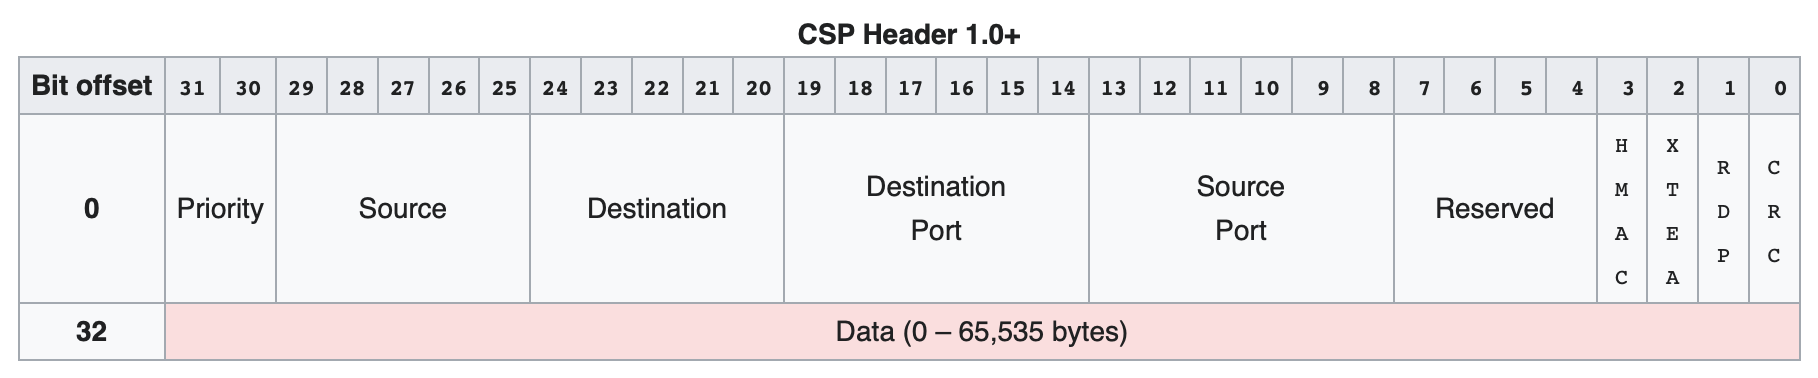
\includegraphics[width=0.9\textwidth]{images/csp_packet}
      \caption{CSP protocol header.}
      \label{fig:csp_packet}
\end{figure}

Both mutations (i.e, header and payload) will be performed before the message is serialized. Particularly, the mutations will affect the csp\_send\_direct function of the csp\_io component.
 

\section{GSL - libparam}
\label{sec:caseStudies:GSL:libparam}

\subsection{Overview of the case study}

The Parameter System (i.e., libparam) is a light-weight parameter system designed for GomSpace satellite subsystems. It is based around a logical memory architecture, where every parameter is referenced directly by its logical address. A backend system takes care of translating addresses into physical addresses.
The features of this system include:
\begin{itemize}
\item Direct memory access for quick parameter reads.
\item Simple data types: uint, int, float, double, string.
\item Arrays of simple data types.
\item Supports multiple stores per table, e.g. FRAM, MCU flash, file (binary or text).
\item Remote client with support for most features (rparam).
\item Packed GET, SET queries, supporting multiple parameter set/get in a single request. ? Data serialization and deserialization.
\item Supports both little and big-endian systems.
\item Commands for both local (param) and remote access (rparam).
\item Parameter server for remote access over CSP.
\item Compile-time configuration of parameter system
\end{itemize}

Details about libparam are provided in the document \emph{gs-man-nanosoft-ms100-command-and-management-sdk-3.6.2-1-g67fe6e1.pdf} uploaded on Alfresco.

\subsection{Code-driven mutation testing}

\TODO{We do it or not?}

\subsection{Data-driven mutation testing}

\TODO{We should indicate the functions we mutate}




\section{GSL - libutil}
\label{sec:caseStudies:GSL:libutil}

\subsection{Overview of the case study}

The Utility library provides cross-platform APIs for common functionality, for use in both embedded systems and standard PCs running Linux. 

Details about libutil are provided in the document \emph{gs-man-nanosoft-ms100-command-and-management-sdk-3.6.2-1-g67fe6e1.pdf} uploaded on Alfresco.

The size of libutil is 10\,576 LOC.

\subsection{Code Coverage}
\label{subsec:libutil_coverage}

% !TEX root = ../MAIN.tex

\begin{table}[h]

\centering
\begin{tabular}{|l|l|}
\hline
\textbf{Coverage Type} & \textbf{Coverage Rate} \\
\hline
Statement     & 83.2\% (8\,817 of 10\,596 statements)\\
Functions     & 82.1\% (725 of 883 functions)\\
Branches      & 56.6\% (2\,618 of 4\,627 branches)\\
\hline
\end{tabular}
\caption{libutil code coverage.}
\label{table:gslibutil_coverage}

\end{table}

Table~\ref{table:gslibutil_coverage} provides the code coverage information of the unit test suite for the GSL libutil library. Given the code coverage, we focus our analysis to the following subset of components:

\begin{itemize}
	\item src/base16.c
	\item src/bytebuffer.c
	\item src/byteorder.c
	\item src/clock.c
	\item src/crc32.c
	\item src/crc8.c
	\item src/error.c
	\item src/fletcher.c
	\item src/function\_scheduler.c
	\item src/hexdump.c
	\item src/lock.c
	\item src/rtc.c
	\item src/string.c
	\item src/strtoint.c
	\item src/time.c
	\item src/timestamp.c
	\item src/cmd/command.c
	\item src/cmd/log.c
	\item src/cmd/vmem.c
	\item src/drivers/sys/memory.c
	\item src/gosh/command.c
	\item src/gosh/console.c
	\item src/gosh/default\_commands.c
	\item src/linux/clock.c
	\item src/linux/command\_line.c
	\item src/linux/cwd.c
	\item src/linux/delay.c
	\item src/linux/function.c
	\item src/linux/mutex.c
	\item src/linux/queue.c
	\item src/linux/rtc.c
	\item src/linux/sem.c
	\item src/linux/signal.c
	\item src/linux/stdio.c
	\item src/linux/thread.c
	\item src/linux/time.c
	\item src/linux/drivers/gpio/gpio.c
	\item src/linux/drivers/gpio/gpio\_sysfs.c
	\item src/linux/drivers/gpio/gpio\_virtual.c
	\item src/linux/drivers/i2c/i2c.c
	\item src/linux/drivers/spi/spi.c
	\item src/linux/drivers/sys/memory.c
	\item src/log/commands.c
	\item src/log/log.c
	\item src/log/appender/console.c
	\item src/log/appender/simple\_file.c
	\item src/test/cmocka.c
	\item src/test/command.c
	\item src/test/log.c
	\item src/vmem/commands.c
	\item src/vmem/vmem.c
	\item src/watchdog/monitor\_task.c
	\item src/watchdog/watchdog.c
	\item src/zip/zip.c
	\item src/zip/miniz/miniz.c
\end{itemize}

\subsection{Code-driven mutation testing}

\DONE{Add some details about what we mutated}

The code-driven mutation testing process in libutil will target all the components covered by the libutil unit test suite. Thus, we include all the components described in the previous Section~\ref{subsec:libutil_coverage}.

\DONE{We can add some preliminary results}

Using the mutation operators AOR, ROR, ICR, LCR, and SDL, we generated 16\,886 mutants. The preliminary results can be found in Table~\ref{table:libutil_preliminary}

% !TEX root = ../MAIN.tex

\begin{table}[h]
\small
\centering
\caption{Code-driven mutation testing preliminary results for the libutil case study.}
\label{table:libutil_preliminary}
\begin{tabular}{|l|l|l|l|l|l|l|}
\hline
        & \multicolumn{5}{c|}{Mutants}                                                                      & \multirow{3}{*}{\begin{tabular}[c]{@{}l@{}}Mutation Score\\ (K/K+L)\end{tabular}} \\ \cline{1-6}
        &     &                                                        &      & \multicolumn{2}{c|}{Killed} &                                                                                   \\ \cline{1-6}
Mutants & All & \begin{tabular}[c]{@{}l@{}}Not\\ Compiled\end{tabular} & Live & Test Failure    & Timeout   &                                                                                   \\ \hline
Total   &  16\,886   &  2\,561                                                      & 3\,402      & 10\,634                & 289          & 76.25\%                                                                           \\ \hline
\end{tabular}
\end{table}    
             

